% !TeX program = xelatex
\documentclass[a4paper,10pt]{article}

% ============================================================================
% សន្លឹកកិច្ចការសិស្សបំពេញចន្លោះ ស-ខ្មៅ និងប្លង់ក្ដារខៀន/ចម្លើយគ្រូ (គ្មាន LCD / គ្មានកន្ត្រៃ)
% មេរៀនទី១ (៤.២)៖ វិធីគុណនិងវិធីចែកចំនួនគត់ — ត្រូវគ្នា ១០០% នឹង LS_Plan_WN13.tex
% ============================================================================
\usepackage[a4paper, left=1.0cm, right=1.0cm, top=0.75cm, bottom=1.00cm, footskip=0.52cm]{geometry}
\usepackage{amsmath}
\usepackage{unicode-math}
\usepackage{fontspec}
\usepackage{array, colortbl}
\usepackage[table]{xcolor}
\usepackage{enumitem}
\usepackage{pifont}
\usepackage{fancyhdr}
\usepackage{lastpage}
\usepackage{tikz}
\usepackage[most]{tcolorbox}
\usetikzlibrary{calc, arrows.meta, decorations.pathreplacing, positioning, babel}

\makeatletter
\let\@expl@@@mark@update@singlecol@structures@@\relax
\makeatother

\providecommand{\NGSFindFonts}{%
  \IfFileExists{C:/Windows/Fonts/cambria.ttc}{%
    \def\NGSSysPath{C:/Windows/Fonts/}%
    \def\NGSUserPath{C:/Users/KIT/AppData/Local/Microsoft/Windows/Fonts/}%
  }{%
    \IfFileExists{./fonts/KhmerOSsiemreap.ttf}{\def\NGSSysPath{./fonts/}\def\NGSUserPath{./fonts/}}{%
    \IfFileExists{../fonts/KhmerOSsiemreap.ttf}{\def\NGSSysPath{../fonts/}\def\NGSUserPath{../fonts/}}{%
    \IfFileExists{../../fonts/KhmerOSsiemreap.ttf}{\def\NGSSysPath{../../fonts/}\def\NGSUserPath{../../fonts/}}{%
    \IfFileExists{../../../fonts/KhmerOSsiemreap.ttf}{\def\NGSSysPath{../../../fonts/}\def\NGSUserPath{../../../fonts/}}{%
    \IfFileExists{../../../../fonts/KhmerOSsiemreap.ttf}{\def\NGSSysPath{../../../../fonts/}\def\NGSUserPath{../../../../fonts/}}{%
    \IfFileExists{../../../../../fonts/KhmerOSsiemreap.ttf}{\def\NGSSysPath{../../../../../fonts/}\def\NGSUserPath{../../../../../fonts/}}{%
    \IfFileExists{../../../../../../fonts/KhmerOSsiemreap.ttf}{\def\NGSSysPath{../../../../../../fonts/}\def\NGSUserPath{../../../../../../fonts/}}{%
      \def\NGSSysPath{../../../../../../../fonts/}\def\NGSUserPath{../../../../../../../fonts/}%
    }}}}}}}%
  }%
}
\NGSFindFonts

\setmathfont[Path={\NGSSysPath}, FontIndex=1, Scale=1.02]{cambria.ttc}
\defaultfontfeatures{Ligatures=TeX}

\setmainfont[
  Path={\NGSUserPath}, Extension=.ttf, Script=Khmer,
  BoldFont={KhmerOSsiemreap}, BoldFeatures={FakeBold=1.8},
  ItalicFont={KhmerOSsiemreap}, ItalicFeatures={FakeSlant=0.25},
  BoldItalicFont={KhmerOSsiemreap}, BoldItalicFeatures={FakeBold=1.8, FakeSlant=0.25}
]{KhmerOSsiemreap}

\newfontfamily\muol[Path={\NGSUserPath}, Extension=.ttf, Script=Khmer]{KhmerOSmuollight}
\newfontfamily\TimesEn[Path={\NGSSysPath}, Extension=.ttf, BoldFont={timesbd}, ItalicFont={timesi}, BoldItalicFont={timesbi}]{times}
\newfontfamily\CalibriFont[Path={\NGSSysPath}, Extension=.ttf]{calibri}

\XeTeXlinebreaklocale "km"
\XeTeXlinebreakskip = 0pt plus 1pt minus 0.1pt

\definecolor{panelgray}{gray}{0.94}
\definecolor{headgray}{gray}{0.85}

\pagestyle{fancy}
\fancyhf{}
\renewcommand{\headrulewidth}{0pt}
\fancyfoot[L]{\fontsize{7.4pt}{9.5pt}\selectfont អនុវិទ្យាល័យព្រះក្រសាំង \en{|} គ្រូ៖ ហុក ប៊ុនថែន \en{|} មេរៀនទី១ (៤.២) វិធីគុណនិងវិធីចែកចំនួនគត់ \en{|} ថ្ងៃព្រហស្បតិ៍ ទី៥ ខែវិច្ឆិកា ឆ្នាំ២០២៦}
\fancyfoot[R]{\fontsize{7.8pt}{10pt}\selectfont ទំព័រ \en{\thepage\ / \pageref{LastPage}}}

\setlength{\parindent}{0pt}
\setlength{\parskip}{0pt}
\setlength{\tabcolsep}{4pt}
\newcolumntype{L}[1]{>{\raggedright\arraybackslash}p{#1}}
\newcolumntype{C}[1]{>{\centering\arraybackslash}p{#1}}

\newcommand{\en}[1]{{\TimesEn #1}}
\newcommand{\enbf}[1]{{\TimesEn\bfseries #1}}
\newcommand{\unit}[1]{\,\text{\en{#1}}}
\newcommand{\cnum}[1]{\mbox{\fontsize{10pt}{12pt}\selectfont\ding{\numexpr181+#1\relax}}}
\newcommand{\chkbox}{\tikz[baseline=-0.15ex]\draw[black, line width=0.85pt, fill=white] (0,0) rectangle (0.24cm,0.24cm);}
\newcommand{\ansbox}[1][1.75cm]{\,\tikz[baseline=-0.65ex]\draw[black, line width=0.65pt, fill=white] (0,0) rectangle (#1, 0.42cm);\,}
\newcommand{\dotline}[1][2.2cm]{\makebox[#1]{\dotfill}}

\newcommand{\pagebanner}[2]{%
  \begin{tcolorbox}[
    enhanced, sharp corners, colback=headgray, colframe=black,
    boxrule=1.05pt, boxsep=1pt, top=2.5pt, bottom=2.5pt, left=6pt, right=6pt,
    after skip=3.5pt
  ]
    {\muol\fontsize{9.0pt}{13.2pt}\selectfont #1}\hfill{\fontsize{8.0pt}{11.2pt}\selectfont\textbf{#2}}
  \end{tcolorbox}%
}

\newcommand{\secstrip}[2]{%
  \vspace{3pt}%
  \begin{tcolorbox}[
    enhanced, sharp corners, colback=panelgray, colframe=black,
    boxrule=0.8pt, boxsep=0.8pt, top=2pt, bottom=2pt, left=5pt, right=5pt,
    after skip=3pt
  ]
    {\muol\fontsize{8.5pt}{12.2pt}\selectfont #1}\hfill{\fontsize{7.8pt}{10.8pt}\selectfont\textit{#2}}
  \end{tcolorbox}%
}

\begin{document}
\fontsize{9.5pt}{14.5pt}\selectfont

% ============================================================================
% ទំព័រទី ១៖ សន្លឹកកិច្ចការសិស្ស (ផ្នែកមុខ៖ E1 -> E2 -> E3)
% ============================================================================
\pagebanner{សន្លឹកកិច្ចការសិស្ស \enbf{(}៤\enbf{.}២ វិធីគុណនិងវិធីចែកចំនួនគត់\enbf{)} \enbf{--} ផ្នែកមុខ}{ថ្នាក់ទី៧ \en{|} សៀវភៅគោល ទំ.៤--៦}

\begin{tcolorbox}[
  enhanced, sharp corners, colback=white, colframe=black,
  boxrule=0.8pt, boxsep=1.5pt, top=3.5pt, bottom=3.5pt, left=5pt, right=5pt,
  after skip=4pt
]
  \fontsize{9.0pt}{13.0pt}\selectfont
  \textbf{ឈ្មោះសិស្ស៖} \dotline[4.3cm] \quad
  \textbf{សមាជិកក្រុម៖} \dotline[4.3cm] \quad
  \textbf{ថ្នាក់ទី៖} ៧\dotline[0.9cm] \quad
  \textbf{ក្រុមទី៖} \dotline[1.0cm]
\end{tcolorbox}

% --- E1 Engage ---
\secstrip{ផ្នែកទី ១ \enbf{(E1 - Engage)} ៖ បេសកកម្មអន្ទាក់ផលគុណរងក្នុង $7\,428 \times 64$}{រយៈពេល ៣ នាទី (គូស \ding{51} ក្នុង \chkbox)}

\begin{tcolorbox}[
  enhanced, sharp corners, colback=white, colframe=black,
  boxrule=0.8pt, boxsep=2pt, top=4pt, bottom=4pt, left=6pt, right=6pt
]
  ក្នុងការគណនាផលគុណ $7\,428 \times 64$ (ឧទាហរណ៍ ២ ទំ.៥) សិស្សពីរនាក់សរសេរផលគុណរងខុសគ្នា៖\\[3pt]
  $\bullet$ \textbf{តើសិស្សរូបណាគណនាបានត្រឹមត្រូវ?} \quad
  \chkbox\ \textbf{សិស្ស ក៖} $29\,712 + 44\,568 = 74\,280$ \quad
  \chkbox\ \textbf{សិស្ស ខ៖} $29\,712 + 445\,680 = 475\,392$\\[3pt]
  $\bullet$ \textbf{ហេតុផល៖} លេខ $6$ ក្នុង $64$ ឈរនៅខ្ទង់ \dotline[1.6cm] មានតម្លៃស្មើនឹង \dotline[1.4cm] ។
\end{tcolorbox}

\vfill

% --- E2 Explore ---
\secstrip{ផ្នែកទី ២ \enbf{(E2 - Explore)} ៖ ផលគុណរងតាមខ្ទង់ និងសមភាពវិធីចែកអឺគ្លីត (ទំ.៥)}{រយៈពេល ១១ នាទី}

\textbf{សកម្មភាព ១ (\en{E2-A} — ៥ នាទី)៖ ការបំបែកផលគុណរងតាមតម្លៃខ្ទង់ (ឧទាហរណ៍ ១--២ ទំ.៤--៥)}

\begin{tcolorbox}[
  enhanced, sharp corners, colback=white, colframe=black,
  boxrule=0.8pt, boxsep=2.5pt, top=4.5pt, bottom=4.5pt, left=6pt, right=6pt
]
  $\bullet$ \textbf{ឧទាហរណ៍ ១ (ទំ.៤)៖} ចំនួនបន្ទះនំប៉័ងអាំង $3 + 3 + 3 + 3 = 4 \times$ \dotline[0.9cm] $=$ \ansbox[1.4cm] បន្ទះ ។\\[3.5pt]
  $\bullet$ \textbf{ឧទាហរណ៍ ២ (ទំ.៥ — គណនា $7\,428 \times 64$ ដោយបំបែក $64 = 60 + 4$)៖}\\[3pt]
  \hspace*{0.3cm}ផលគុណរងទី១ ($7\,428 \times 4$) $=$ \dotline[2.2cm] \quad
  ផលគុណរងទី២ ($7\,428 \times 60$) $=$ \dotline[2.4cm] $\implies$ សរុប $=$ \ansbox[2.4cm]
\end{tcolorbox}

\vspace{4pt}
\textbf{សកម្មភាព ២ (\en{E2-B} — ៦ នាទី)៖ វិធីចែកដាច់ និងវិធីចែកមានសំណល់ (ឧទាហរណ៍ ៣--៤ ទំ.៥)}

\begin{tcolorbox}[
  enhanced, sharp corners, colback=white, colframe=black,
  boxrule=0.8pt, boxsep=2.5pt, top=4.5pt, bottom=4.5pt, left=6pt, right=6pt
]
  $\bullet$ \textbf{ឧទាហរណ៍ ៤ ក (ទំ.៥)៖} $6\,645 \div 15 \to$ ផលចែក $q =$ \dotline[1.4cm], សំណល់ $r =$ \dotline[1.0cm] $\implies 6\,645 = 15 \times$ \dotline[1.4cm] $+ 0$ ។\\[3.5pt]
  $\bullet$ \textbf{ឧទាហរណ៍ ៤ ខ (ទំ.៥)៖} $5\,406 \div 128 \to$ ផលចែក $q =$ \ansbox[1.4cm], សំណល់ $r =$ \ansbox[1.4cm] (ផ្ទៀង៖ $r < 128$ \chkbox)\\[3pt]
  \hspace*{0.3cm}ផ្ទៀងផ្ទាត់សមភាពអឺគ្លីត៖ $128 \times 42 + 30 =$ \dotline[1.8cm] $+ 30 =$ \ansbox[1.9cm] ។
\end{tcolorbox}

\vfill

% --- E3 Explain ---
\secstrip{ផ្នែកទី ៣ \enbf{(E3 - Explain)} ៖ ទំនាក់ទំនងច្រាស សមភាពអឺគ្លីត និងធនាគារហេតុផល \enbf{B\&W}}{រយៈពេល ៦ នាទី}

\begin{tcolorbox}[
  enhanced, sharp corners, colback=white, colframe=black,
  boxrule=0.85pt, boxsep=2.5pt, top=4pt, bottom=4pt, left=6pt, right=6pt
]
  ១) បើ $a \times b = c$ ($a\ne 0, b\ne 0$) នោះ $a = c \div$ \dotline[0.8cm] និង $b = c \div$ \dotline[0.8cm] \quad
  ២) វិធីចែកមានសំណល់៖ $D = d \times$ \dotline[0.8cm] $+$ \dotline[0.8cm] ($0 \le r < d$)\\[4pt]
  \tikz\draw[black, dashed, line width=0.5pt] (0,0) -- (18.4cm,0);\\[3.5pt]
  \fontsize{8.8pt}{13.0pt}\selectfont
  \textbf{ធនាគារហេតុផល (\en{Warrant Bank})៖} \quad
  \cnum{1} \textbf{ផលគុណរងតាមខ្ទង់៖} គុណនឹងខ្ទង់ដប់ត្រូវរំកិលមួយខ្ទង់មកឆ្វេង (ថែម $0$ នៅខ្ទង់រាយ)\\
  \cnum{2} \textbf{វិធីចែកអឺគ្លីត៖} $D = d \times q + r$ ដែល $0 \le r < d$ \quad
  \cnum{3} \textbf{វិធានច្រាស៖} $a = c \div b$ \quad
  \cnum{4} \textbf{ចំណោទ៖} ច្រំដែលស្មើគ្នា $\to \times$; ចែកស្មើគ្នា $\to \div$
\end{tcolorbox}

% ============================================================================
% ទំព័រទី ២៖ សន្លឹកកិច្ចការសិស្ស (ផ្នែកខាងខ្នង៖ E4 -> E5 -> កិច្ចការផ្ទះ)
% ============================================================================
\clearpage
\pagebanner{សន្លឹកកិច្ចការសិស្ស \enbf{(}៤\enbf{.}២ វិធីគុណនិងវិធីចែកចំនួនគត់\enbf{)} \enbf{--} ផ្នែកខាងខ្នង}{ថ្នាក់ទី៧ \en{|} សៀវភៅគោល ទំ.៦ និង ទំ.១៤}

% --- E4 Elaborate ---
\secstrip{ផ្នែកទី ៤ \enbf{(E4 - Elaborate)} ៖ លំហាត់គំរូ ១ និង ២ — បណ្ណាគារ និងការបែងចែកតុសិស្ស (ទំ.៦)}{រយៈពេល ១០ នាទី}

\begin{tcolorbox}[
  enhanced, sharp corners, colback=white, colframe=black,
  boxrule=0.8pt, boxsep=2.5pt, top=4.5pt, bottom=4.5pt, left=6pt, right=6pt
]
  $\bullet$ \textbf{លំហាត់គំរូ ១ (ទំ.៦)៖} បណ្ណាគារមួយលក់សៀវភៅក្នុងមួយថ្ងៃបាន $85$ ក្បាល ។ តើក្នុងរយៈពេលពីរសប្ដាហ៍ បណ្ណាគារនោះនឹងលក់សៀវភៅបានប៉ុន្មានក្បាល បើក្នុងមួយថ្ងៃៗលក់បានសៀវភៅស្មើគ្នា?\\[3pt]
  \hspace*{0.3cm}បំបែករយៈពេល៖ $2\text{ សប្ដាហ៍} = 2 \times 7 =$ \dotline[1.2cm] ថ្ងៃ $\implies$ សៀវភៅសរុប៖ $85 \times$ \dotline[1.2cm] $=$ \ansbox[2.2cm] ក្បាល ។\\[4pt]
  $\bullet$ \textbf{លំហាត់គំរូ ២ (ទំ.៦)៖} សាលារៀនមួយមាន $32$ បន្ទប់ និងមានតុសិស្សចំនួន $1\,280$ ។ បើបន្ទប់រៀននីមួយៗមានចំនួនតុស្មើគ្នា រកចំនួនតុសិស្សសម្រាប់បន្ទប់រៀននីមួយៗ ៖\\[3pt]
  \hspace*{0.3cm}ចំនួនតុក្នុង ១ បន្ទប់៖ $1\,280 \div 32 =$ \ansbox[2.0cm] តុ \quad (ផ្ទៀងផ្ទាត់ច្រាស \cnum{3}៖ $32 \times$ \dotline[1.3cm] $= 1\,280$ តុ) ។\\[3pt]
  \fontsize{8.8pt}{12.8pt}\selectfont
  \textbf{ឆ្លុះបញ្ចាំង (\en{EIA Looking-Back})៖} បើមានតុ $1\,295$ តុ ចែកដាក់ក្នុង $32$ បន្ទប់ស្មើគ្នា នោះក្នុង ១ បន្ទប់បាន $40$ តុ និងនៅសល់សំណល់ $r =$ \dotline[1.2cm] តុ ។
\end{tcolorbox}

\vfill

% --- E5 Evaluate ---
\secstrip{ផ្នែកទី ៥ \enbf{(E5 - Evaluate)} ៖ លំហាត់ប្រតិបត្តិ (ទំ.៦) សំណួរវិនិច្ឆ័យ \enbf{A--D} និងសំបុត្រចេញ}{រយៈពេល ១០ នាទី}

\begin{tcolorbox}[
  enhanced, sharp corners, colback=white, colframe=black,
  boxrule=0.8pt, boxsep=2.5pt, top=4.5pt, bottom=4.5pt, left=6pt, right=6pt
]
  \textbf{១) ប្រតិបត្តិជាក្រុមតូច ៣ នាក់ — ចូរធ្វើវិធីចែក និងវិធីគុណខាងក្រោម (សៀវភៅគោល ទំ.៦)៖}\\[4pt]
  $\bullet$ \textbf{ក.} $669\,292 \div 122 =$ \ansbox[2.5cm] \qquad (ផ្ទៀងផ្ទាត់៖ $122 \times$ \dotline[2.0cm] $= 669\,292$)\\[4.5pt]
  $\bullet$ \textbf{ខ.} $7\,769 \times 324 \times 189 =$ \dotline[3.0cm] $\times 189 =$ \ansbox[3.2cm]\\[4.5pt]
  \textbf{២) បិទបេសកកម្ម \en{E1}៖} សិស្ស \dotline[1.0cm] ត្រឹមត្រូវ ព្រោះ $7\,428 \times 60 =$ \dotline[2.0cm] ដូច្នេះ $7\,428 \times 64 =$ \dotline[2.0cm] ។
\end{tcolorbox}

\vspace{4pt}

\begin{tcolorbox}[
  enhanced, sharp corners, colback=white, colframe=black,
  boxrule=0.8pt, boxsep=2.5pt, top=4.5pt, bottom=4.5pt, left=6pt, right=6pt
]
  \textbf{៣) សំណួរវិនិច្ឆ័យ \en{A--D} (តើផលចែក $q$ និងសំណល់ $r$ នៃ $380 \div 25$ ស្មើនឹងប៉ុន្មាន? — គូសរង្វង់ រួចលើកម្រាមដៃ ១--៤)៖}\\[3.5pt]
  \textbf{\en{A.}} $q = 14, \ r = 30$ \qquad\quad
  \textbf{\en{B.}} $q = 15, \ r = 15$ \qquad\quad
  \textbf{\en{C.}} $q = 15, \ r = 5$ \qquad\quad
  \textbf{\en{D.}} $q = 16, \ r = 20$\\[4.5pt]
  \tikz\draw[black, dashed, line width=0.5pt] (0,0) -- (18.4cm,0);\\[3.5pt]
  \textbf{៤) សំបុត្រចេញ ៦០ វិនាទី៖} តាមទំនាក់ទំនងច្រាស (\cnum{3}) បើ $a \times 16 = 480$ នោះ $a = 480 \div 16 =$ \ansbox[1.8cm] ។
\end{tcolorbox}

\vfill

% --- Homework ---
\begin{tcolorbox}[
  enhanced, sharp corners, colback=panelgray, colframe=black,
  boxrule=0.95pt, boxsep=2.5pt, top=4pt, bottom=4pt, left=6pt, right=6pt
]
  {\muol\fontsize{9.0pt}{13.0pt}\selectfont កិច្ចការផ្ទះ \enbf{(}សៀវភៅគោល ទំ.១៤ លេខ ៤ និង លេខ ៥\enbf{)}}\\[3pt]
  \fontsize{8.8pt}{12.8pt}\selectfont
  $\bullet$ \textbf{លេខ ៤៖} ប៊ុនណាបានទិញផ្លែមៀន $5$ ចង្កោម ដែលក្នុងមួយចង្កោមមាន $10$ ផ្លែ ។ គាត់បានញ៉ាំអស់ $8$ ផ្លែ ហើយផ្លែមៀននៅសល់បានបែងចែកឱ្យប្អូនៗគាត់ $6$ នាក់ ។ តើប្អូនគាត់ម្នាក់ៗទទួលបានមៀនប៉ុន្មានផ្លែ?\\[2pt]
  $\bullet$ \textbf{លេខ ៥៖} នៅក្នុងថ្នាក់រៀនមួយមានសិស្សប្រុស $18$ នាក់និងសិស្សស្រីខ្លះ ។ បើសិស្សម្នាក់ៗទទួលបានសៀវភៅលំហាត់ $2$ ក្បាល ហើយសៀវភៅលំហាត់ដែលបានទិញទាំងអស់មានចំនួន $76$ ក្បាល ។ រកចំនួនសិស្សស្រី ។
\end{tcolorbox}

% ============================================================================
% ទំព័រទី ៣៖ ទំព័រគ្រូបង្រៀន (គំរូប្លង់ក្ដារខៀន ៣ ផ្នែក + ចម្លើយផ្ទៀងផ្ទាត់រហ័ស)
% ============================================================================
\clearpage
\pagebanner{ទំព័រគ្រូបង្រៀន ៖ ប្លង់ក្ដារខៀន \enbf{(}គ្មាន \enbf{LCD)} និងចម្លើយផ្ទៀងផ្ទាត់រហ័ស}{៤.២ វិធីគុណនិងវិធីចែកចំនួនគត់ (\en{WN13})}

\secstrip{១. គំរូប្លង់បែងចែកក្ដារខៀន ៣ ផ្នែក សម្រាប់ថ្នាក់រៀនគ្មាន \enbf{LCD}}{សម្រាប់គ្រូប្រើដីស/ហ្វឺត}

\begin{center}
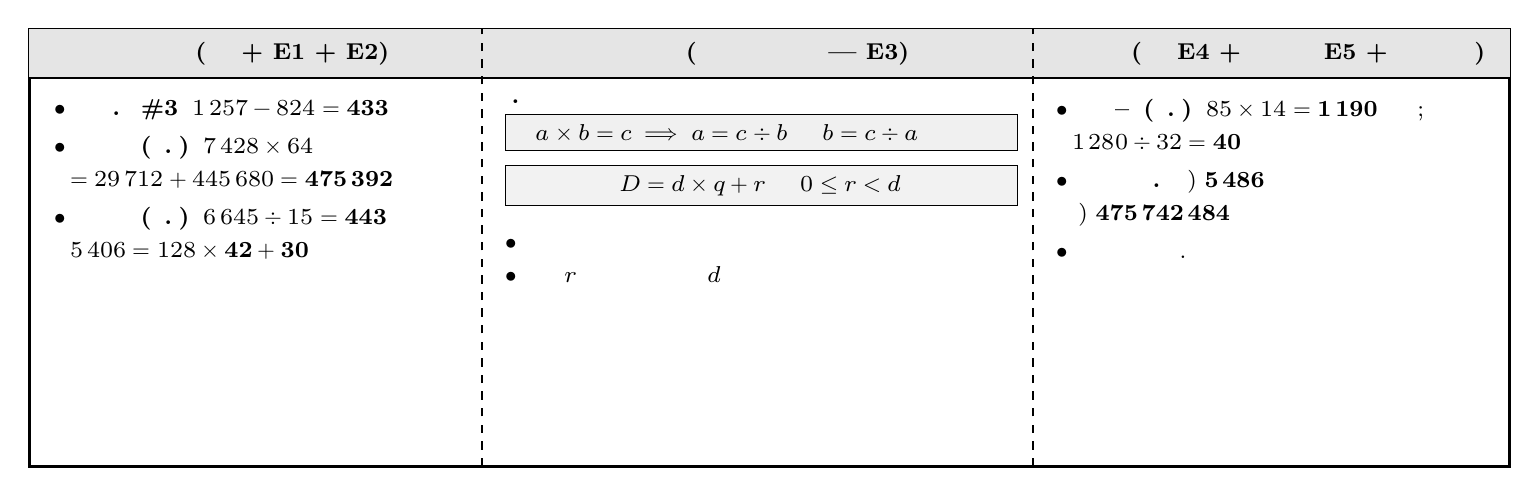
\begin{tikzpicture}[x=1cm, y=1cm, every node/.style={font=\fontsize{8.3pt}{11.8pt}\selectfont, text=black}]
  \draw[black, line width=1.1pt] (0,0) rectangle (18.8,5.55);
  \fill[gray!20] (0,4.93) rectangle (18.8,5.55);
  \draw[black, line width=0.7pt] (0,4.93) -- (18.8,4.93);
  \draw[black, dashed, line width=0.7pt] (5.75,0) -- (5.75,5.55);
  \draw[black, dashed, line width=0.7pt] (12.75,0) -- (12.75,5.55);

  \node at (2.875,5.24) {\textbf{ផ្នែកឆ្វេង (កំណែ + \en{E1} + \en{E2})}};
  \node at (9.25,5.24) {\textbf{ផ្នែកកណ្ដាល (ខ្លឹមសារគោលរក្សាទុក — \en{E3})}};
  \node at (15.775,5.24) {\textbf{ផ្នែកស្ដាំ (គំរូ \en{E4} + ប្រតិបត្តិ \en{E5} + កិច្ចការផ្ទះ)}};

  % Left
  \node[anchor=north west, text width=5.35cm] at (0.20,4.78) {%
    $\bullet$ \textbf{កំណែទំ.១៤ \#3៖} $1\,257 - 824 = \mathbf{433}$ នាក់\\[2pt]
    $\bullet$ \textbf{ឧទាហរណ៍ ២ (ទំ.៥)៖} $7\,428 \times 64$\\
    \hspace*{0.2cm}$= 29\,712 + 445\,680 = \mathbf{475\,392}$\\[2pt]
    $\bullet$ \textbf{ឧទាហរណ៍ ៤ (ទំ.៥)៖} $6\,645\div 15 = \mathbf{443}$\\
    \hspace*{0.2cm}$5\,406 = 128 \times \mathbf{42} + \mathbf{30}$
  };

  % Center
  \node[anchor=north west, text width=6.65cm] at (5.92,4.78) {%
    {\muol\fontsize{8.5pt}{12pt}\selectfont ៤\enbf{.}២ វិធីគុណនិងវិធីចែកចំនួនគត់}\\[3pt]
    \tikz\node[draw=black, fill=gray!12, inner sep=3.5pt, text width=6.25cm]{%
      បើ $a \times b = c \implies a = c \div b$ និង $b = c \div a$
    };\\[4pt]
    \tikz\node[draw=black, fill=gray!10, inner sep=3.5pt, text width=6.25cm]{%
      វិធីចែកអឺគ្លីត៖ $D = d \times q + r$ ដែល $0 \le r < d$
    };\\[4pt]
    $\bullet$ គុណនឹងខ្ទង់ដប់ត្រូវរំកិល ១ ខ្ទង់មកឆ្វេង\\
    $\bullet$ សំណល់ $r$ ត្រូវតែតូចជាងតួចែក $d$ ជានិច្ច
  };

  % Right
  \node[anchor=north west, text width=5.65cm] at (12.92,4.78) {%
    $\bullet$ \textbf{គំរូ ១–២ (ទំ.៦)៖} $85 \times 14 = \mathbf{1\,190}$ ក្បាល;\\
    \hspace*{0.2cm}$1\,280 \div 32 = \mathbf{40}$ តុ\\[2pt]
    $\bullet$ \textbf{ប្រតិបត្តិទំ.៦៖} ក) $\mathbf{5\,486}$\\
    \hspace*{0.2cm}ខ) $\mathbf{475\,742\,484}$\\[2pt]
    $\bullet$ \textbf{កិច្ចការផ្ទះ៖} ទំ.១៤ លេខ ៤ និង លេខ ៥
  };
\end{tikzpicture}
\end{center}

\vfill
\secstrip{២. ចម្លើយផ្ទៀងផ្ទាត់រហ័សសម្រាប់សន្លឹកកិច្ចការសិស្ស \enbf{(}ទំព័រ ១ និង ទំព័រ ២\enbf{)}}{\en{Answer Key}}

\begin{tcolorbox}[
  enhanced, sharp corners, colback=white, colframe=black,
  boxrule=0.8pt, boxsep=2.5pt, top=4.5pt, bottom=4.5pt, left=6pt, right=6pt
]
  \fontsize{9.0pt}{13.5pt}\selectfont
  $\bullet$ \textbf{ផ្នែក \en{E1}៖} \textbf{សិស្ស ខ} ត្រឹមត្រូវ ($475\,392$) ព្រោះលេខ $6$ ឈរនៅខ្ទង់ដប់ មានតម្លៃស្មើនឹង $60$ ។\\[2pt]
  $\bullet$ \textbf{ផ្នែក \en{E2}៖} \textbf{សកម្មភាព ១៖} $4\times 3 = 12$; $29\,712 + 445\,680 = 475\,392$ ។ \textbf{សកម្មភាព ២៖} ក) $q=443, r=0$; ខ) $q=42, r=30 \implies 5\,376 + 30 = 5\,406$ ។\\[2pt]
  $\bullet$ \textbf{ផ្នែក \en{E4}៖} គំរូ ១៖ $14$ ថ្ងៃ $\implies 85 \times 14 = 1\,190$ ក្បាល; គំរូ ២៖ $1\,280 \div 32 = 40$ តុ; \en{EIA}៖ សំណល់ $r = 15$ តុ ។\\[2pt]
  $\bullet$ \textbf{ផ្នែក \en{E5}៖} \textbf{១) ប្រតិបត្តិ៖} ក) $5\,486$; ខ) $2\,517\,156 \times 189 = 475\,742\,484$ ។ \textbf{២) បិទ \en{E1}៖} សិស្ស ខ ($445\,680$, $475\,392$) ។ \textbf{៣) វិនិច្ឆ័យ \en{A--D}៖} \textbf{ជម្រើស \en{C}} ($q=15, r=5$) ។ \textbf{៤) សំបុត្រចេញ៖} $a = 30$ ។
\end{tcolorbox}

\vfill
\secstrip{៣. ចម្លើយលម្អិតនៃកិច្ចការផ្ទះ \enbf{(}សៀវភៅគោល ទំ.១៤ លេខ ៤ និង លេខ ៥\enbf{)}}{សៀវភៅគោល ទំ.១៤}

\begin{tcolorbox}[
  enhanced, sharp corners, colback=white, colframe=black,
  boxrule=0.8pt, boxsep=2.5pt, top=4.5pt, bottom=4.5pt, left=6pt, right=6pt
]
  \fontsize{8.9pt}{13.3pt}\selectfont
  $\bullet$ \textbf{លេខ ៤ (ទំ.១៤)៖} មៀនទិញសរុប $= 5 \times 10 = 50$ ផ្លែ; មៀននៅសល់ $= 50 - 8 = 42$ ផ្លែ; ប្អូនម្នាក់ៗទទួលបាន $= 42 \div 6 = \mathbf{7\text{ ផ្លែ}}$ ។\\[2pt]
  $\bullet$ \textbf{លេខ ៥ (ទំ.១៤)៖} ចំនួនសិស្សទាំងអស់ក្នុងថ្នាក់ $= 76 \div 2 = 38$ នាក់; ចំនួនសិស្សស្រី $= 38 - 18 = \mathbf{20\text{ នាក់}}$ (ផ្ទៀង៖ $(18+20)\times 2 = 76$ ក្បាល) ។
\end{tcolorbox}

\vfill
\secstrip{៤. ចំណុចប្រុងប្រយ័ត្នគរុកោសល្យសម្រាប់គ្រូ \enbf{(}ការយល់ច្រឡំសំខាន់ៗ និងកំណត់សម្គាល់សៀវភៅពុម្ព\enbf{)}}{\en{Pedagogical Watchlist}}

\begin{tcolorbox}[
  enhanced, sharp corners, colback=panelgray, colframe=black,
  boxrule=0.85pt, boxsep=2.5pt, top=4.5pt, bottom=4.5pt, left=6pt, right=6pt
]
  \fontsize{8.8pt}{13.1pt}\selectfont
  $\bullet$ \textbf{កំណត់សម្គាល់កំហុសបោះពុម្ពក្នុងសៀវភៅគោលទំ.៥ (ឧទាហរណ៍ ៤ ខ)៖} ប្រធានដាក់ $5\,406 \div 128$ (ឃើញ $q=42, r=30$) ប៉ុន្តែបន្ទាត់សរុបខាងក្រោមបានបោះពុម្ពខុសជា «$5\,408 = 128 \times 42 + 30$» ។ សូមណែនាំសិស្សឱ្យគណនា $128 \times 42 + 30 = 5\,376 + 30 = \mathbf{5\,406}$ ដើម្បីបង្កើនទម្លាប់ផ្ទៀងផ្ទាត់ដោយខ្លួនឯង!\\[2pt]
  $\bullet$ \textbf{អន្ទាក់ប្រតិបត្តិ ខ ($7\,769 \times 324 \times 189$)៖} ត្រូវរំកិលផលគុណរងទី២ (មួយខ្ទង់) និងផលគុណរងទី៣ (ពីរខ្ទង់) ឱ្យត្រង់ជួរឈរ មុននឹងបូកបញ្ចូលគ្នា ។
\end{tcolorbox}

\end{document}
